
This section presents the evaluation results by comparing SQLiteKV with SQLite and SnappyDB, which are representative SQL and Key-value databases, respectively. In this section, we first introduce the experimental setup, then provide the experimental results with real-world benchmarks and synthetic workloads, with the overhead analysis provided at the end \cite{cooper2010benchmarking}.
\section{Experiment Setup}
We have prototyped the proposed SQLiteKV on Google Nexus platform. Our implementation is based on SQLite and SnappyDB, and includes 2,344 lines of code. 

All experiments have been conducted on Google’s Nexus 6p smartphone that has a 2.0 GHz oct-core 64 bit Qualcomm Snapdragon 810 processor, 3 GB LPDDR4 RAM, Samsung-manufactured 32 GB eMMC 5.0 NAND flash and Android 7.1.2 with Linux Kernel 3.10.73.

SQLite 3.9 is utilized in the experiments as this is the current version in Google Nexus 6p. The page size of SQLite is set as 1024 bytes that is the default valud. SnappyDB 0.4.0 is adopted that is the latest version of a java implementation of Google's LevelDB. SQLiteKV is implemented based on the same version of SnappyDB. 

To make a fair comparison, in our experiments, for each SQL query in SQLite, it contains up to 999 variables that is the maximum value allowed. In this way, we avoid unnecessary inefficiency from one benchmark tool ~\cite{SnappyDB} from SnappyDB in which one SQLite query would only carry one variable at one time. Moreover, unnecessary calls like cursor.moveToFirst() after queries are not performed for the sake of efficiency.

\section{Overall Performance}

%To generate real-world key-value requests to the database engine, we adopt a workload model presented in prior work \cite{shen2017didacache}. This model is built based on real workloads \cite{atikoglu2012workload}, and 
Based on the database benchmark tool \cite{cooper2010benchmarking}, we have generated a set of real-world workloads to evaluate the overall performance. The ratio of insertions and queries of each workload is shown in Table ~\ref{table:workload}.
\begin{table}
	\begin{center}
		\caption{Workload  Characteristics.}
		\begin{tabular}{|p{2.5cm}|p{1.5cm}|p{1.5cm}|} 
			\hline
			Workload(s) & Query & Insert \\ 
			\hline
			Update Heavy & 0.5 & 0.5 \\ 
			\hline
			Read Most & 0.95 & 0.05 \\
			\hline
			Read Heavy & 1 & 0 \\
			\hline
			Read Latest & 0.05 & 0.95  \\ 
			\hline
		\end{tabular}
		\label{table:workload}
	\end{center}
\end{table}

To generate real-world requests to the database engines, we first generate 100 thousand key value pairs to populate our databases, and then use the object popularity model to generate 100 thousand SQLite and KV requests, respectively. The object popularity, which determines the request sequence, follows a Zipfian distribution ~\cite{shen2017didacache}, by which some records in the head will be extremely popular while some in the tail are not. In the Read Latest workload, it follows the Zipfian distribution except that most recently inserted records will be in the head of the distribution so they will be accessed more frequently. For all other workloads, record selections follow Zipfian distribution. 
\begin{figure*}
	\centering
	\begin{minipage}[t]{0.4\textwidth}
		\centering
		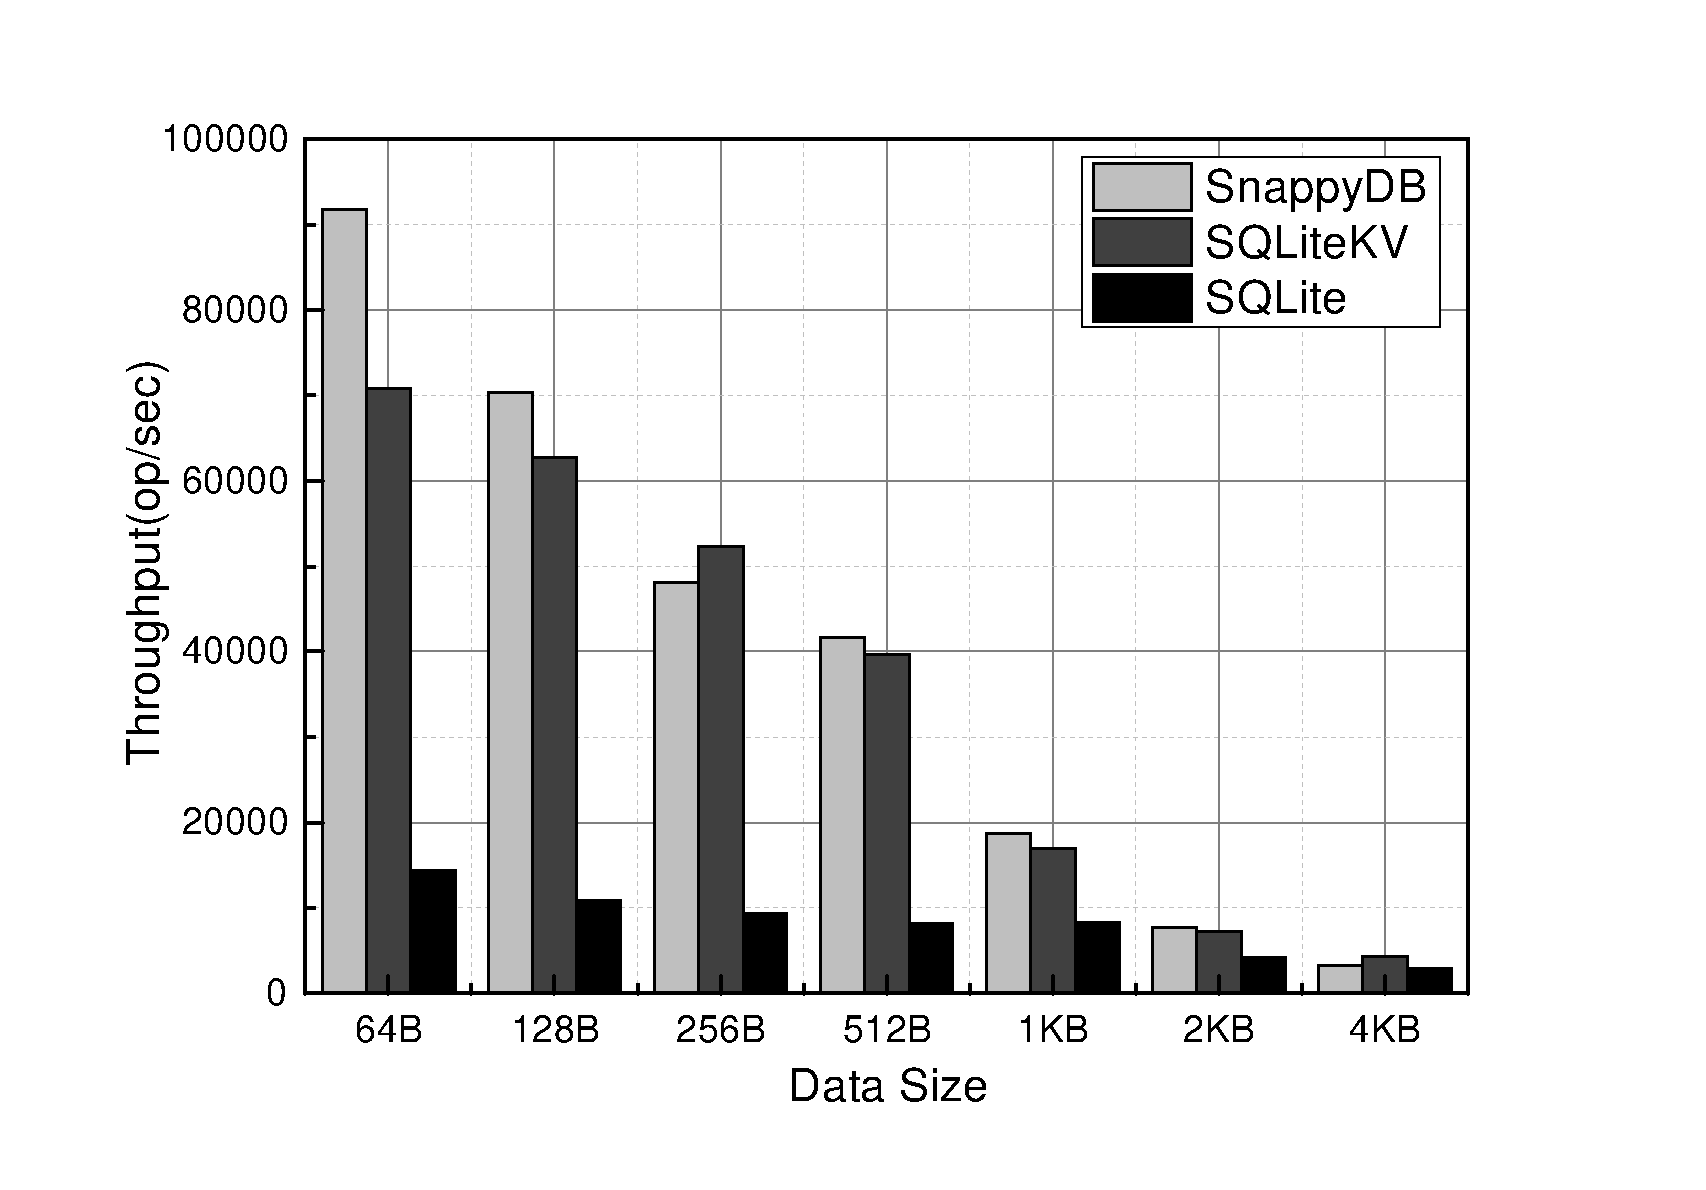
\includegraphics[width=0.9\textwidth, height=3.5cm]{Ext/workload1.pdf}
		\vspace*{-0.2cm}
		\caption{\small Throughput w. Update Heavy Workload.}
		\label{fig:workload1}
	\end{minipage}%
	\hspace*{0.7cm}
	\begin{minipage}[t]{0.4\textwidth}
		\centering
		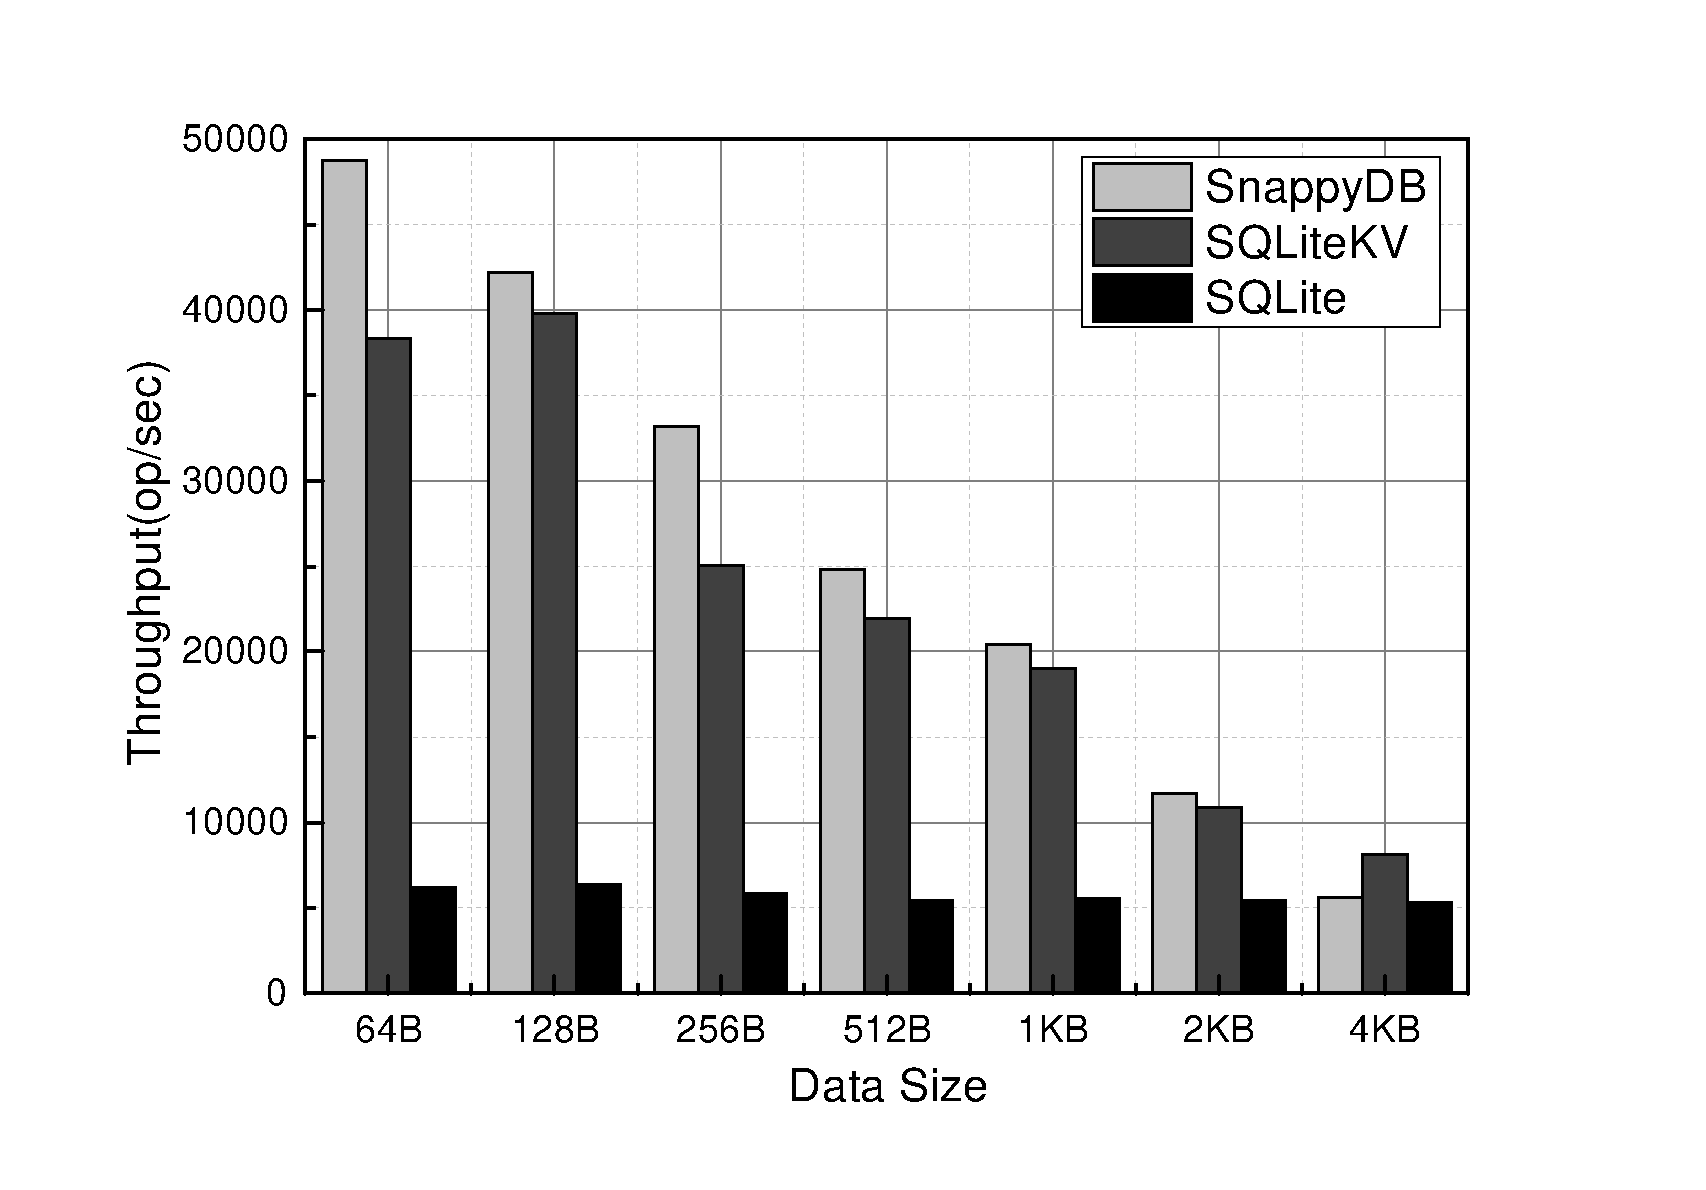
\includegraphics[width=0.9\textwidth, height=3.5cm]{Ext/workload2.pdf}
		\vspace*{-0.2cm}
		\caption{\small Throughput w. Read Most Workload.}
		\label{fig:workload2}
	\end{minipage}
\end{figure*}

\begin{figure*}
	\centering
	\begin{minipage}[t]{0.4\textwidth}
		\centering
		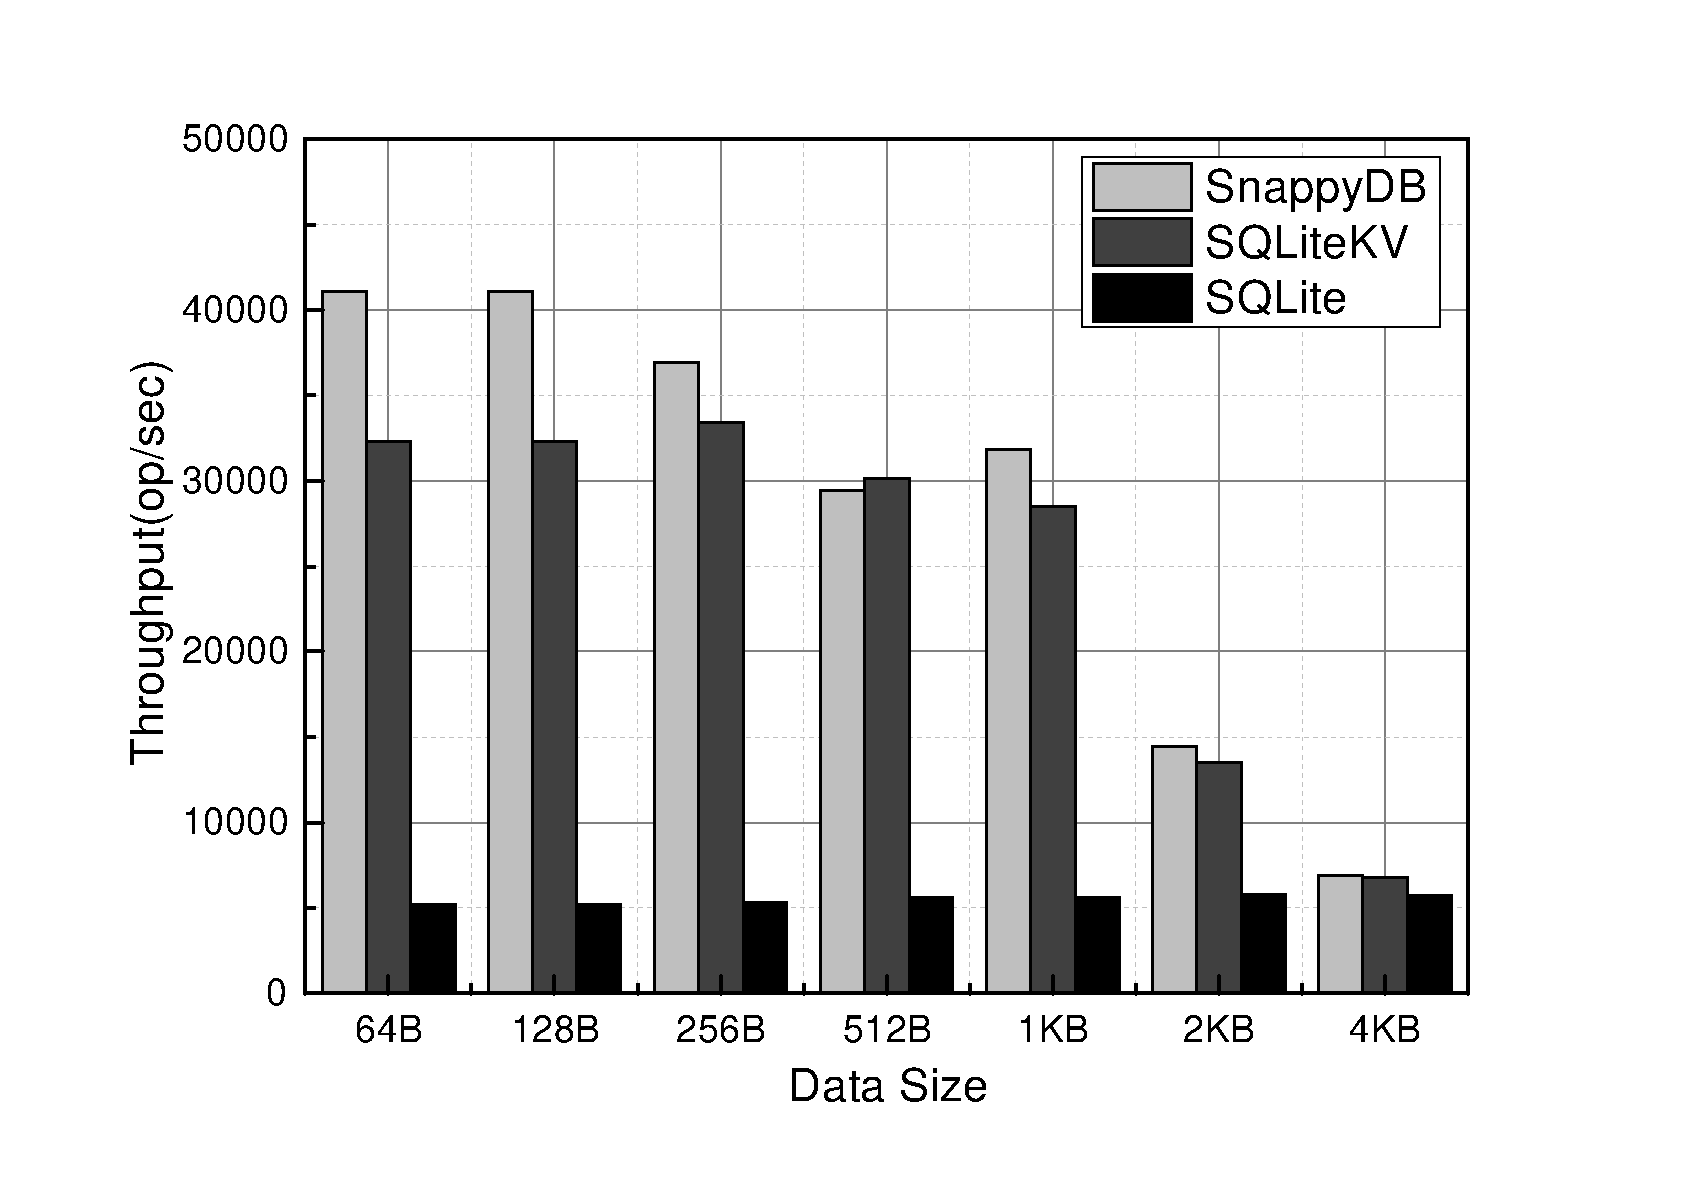
\includegraphics[width=0.9\textwidth, height=3.5cm]{Ext/workload3.pdf}
		\vspace*{-0.2cm}
		\caption{\small Throughput w. Read Heavy Workload.}
		\label{fig:workload3}
	\end{minipage}%
	\hspace*{0.7cm}
	\begin{minipage}[t]{0.4\textwidth}
		\centering
		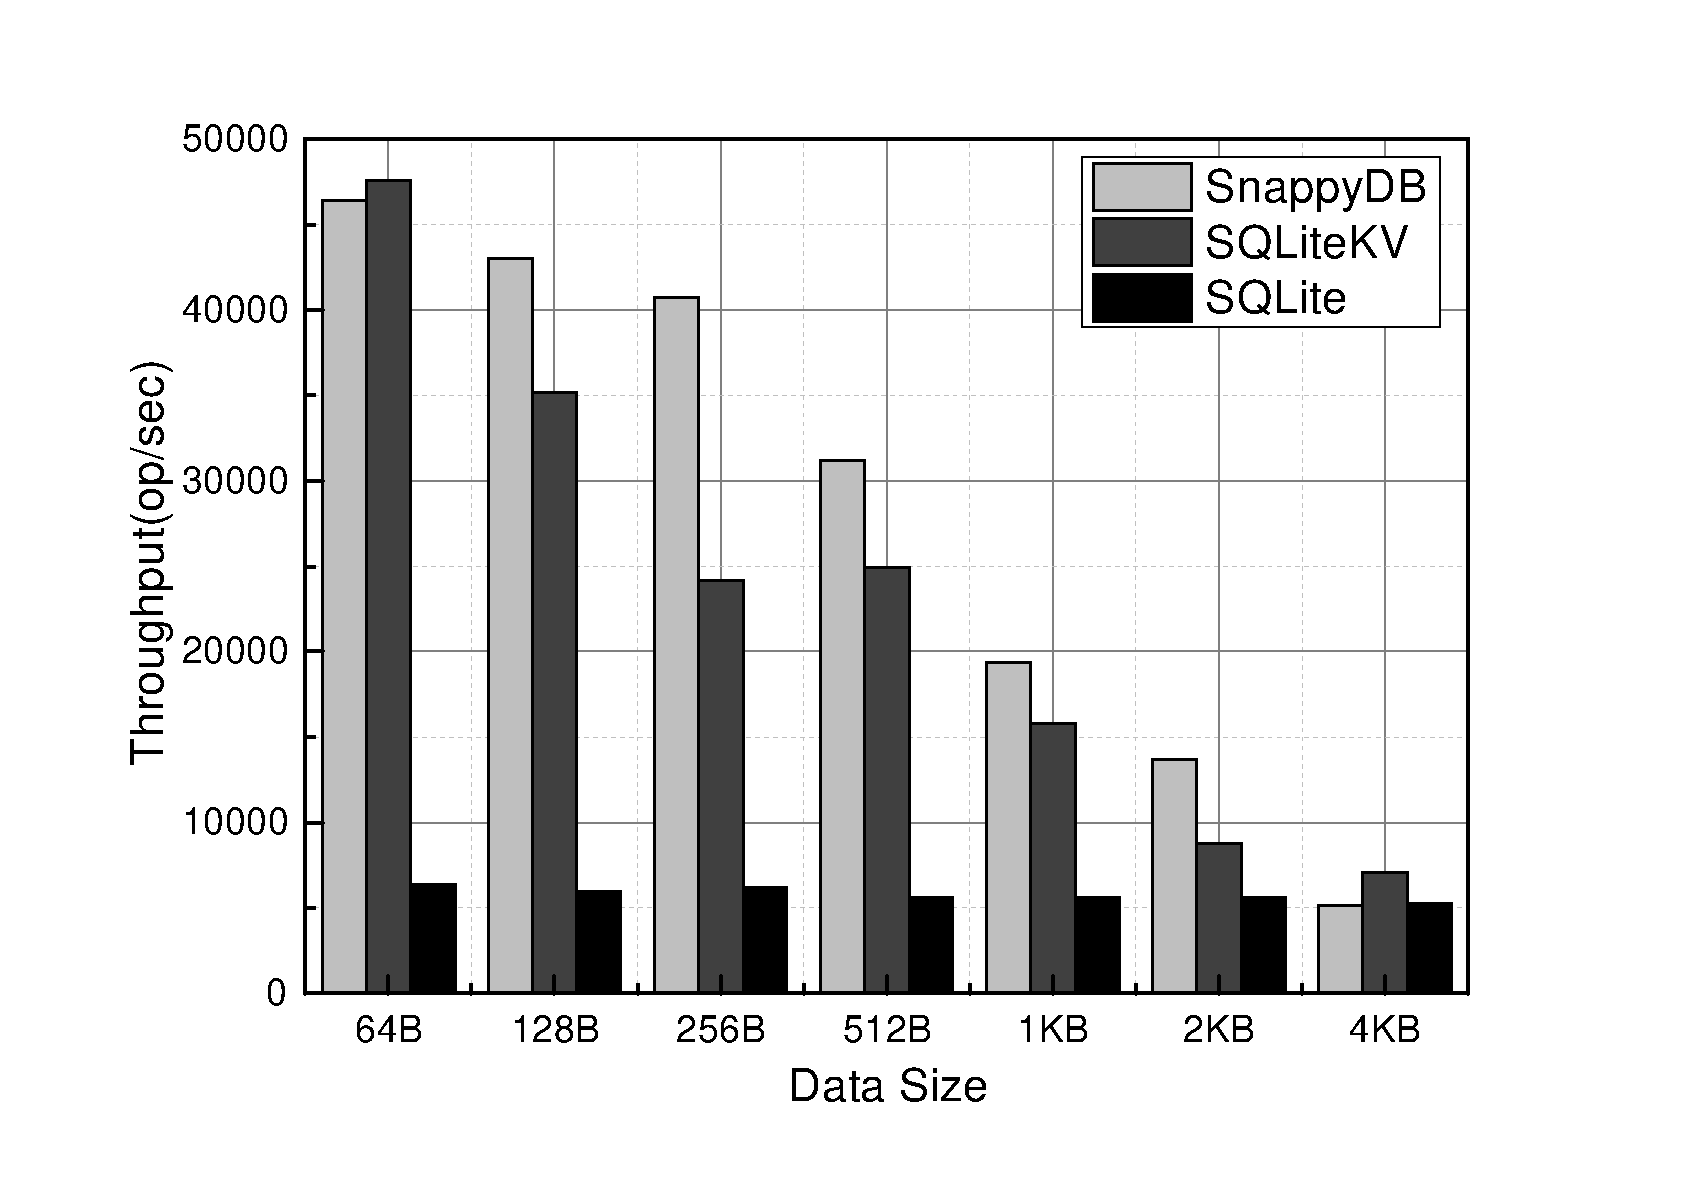
\includegraphics[width=0.9\textwidth, height=3.5cm]{Ext/workload4.pdf}
		\vspace*{-0.2cm}
		\caption{\small Throughput w. Read Latest Workload.}
		\label{fig:workload4}
	\end{minipage}
	
	\caption{\small Overall Performance}
	\label{fig:overallPerformance}
\end{figure*}
Figure \ref{fig:overallPerformance} shows the experimental results by running SnappyDB, SQLiteKV, and SQLite with the four workloads in ~\ref{table:workload}. For each workload, the key-value item sizes vary from 64 bytes to 4096 bytes. It can be observed that when the key-value item size is less than 2048 bytes, compared with SQLite, SQLiteKV significantly increases the throughput (operations per second). For example, the throughput with the 64-byte key-value items is improved by over 6.1 times. At the same time, with the same configuration (64-byte key-value), SQLite introduces from 18.2\% to 40.76\% throughput degradation against SnappyDB. As most data sets in SQLite with mobile applications are dominated with small requests (i.e. less than 100 bytes ~\cite{atikoglu2012workload}), we believe it is worthwhile for SQLiteKV to scarify this overhead while providing a SQLite interface.     

When the key-value sizes are over 2048 bytes, SQLiteKV, as well as SnappyDB, does not significantly outperform SQLite. The reason is that for LSM-tree-based databases, keys and values are written at least twice: the first time for the transactional log and the second time for storing data to storage devices. Thus, the per-operation performance of SQLiteKV is degraded by extra write operations. Regardless of this degradation, since most data sets in mobile applications only contain very few large requests, SQLiteKV can still significantly outperform SQLite in practice.    

To check the influence with the different insertion/query ratios, we use the case with 128-byte KV items as an example. For the Update Heavy workload, for SQLiteKV, the throughput is 20\% higher than that with the Read Heavy workload. The main reason is that in LSM-tree-based databases, for randomness-dominated workloads as these we use, write efficiency is better than read efficiency ~\cite{sears2012blsm}. For SQLiteKV, the similar trends can be observed from other workloads. 

In summary, SQLiteKV can significantly outperform SQLite by over 6 times on throughput for different workloads with various insertion/query ratios when the sizes of requests are small (no more than 128 bytes).  



\section{Performance with Different Sequential/Random Workloads}
In the second set of experiments, we investigate the impact of random and sequential accesses on SQLiteKV, SQLite and SnappyDB. Here, the key size is 16 bytes and the value size varies from 64 bytes to 4096 bytes. Next, we present the results related to insertions and queries, respectively.  

\subsubsection{Insertion Performance}
Figure ~\ref{fig:S-write} shows the results with random and sequential insertion operations, respectively, in which the key-value size varies from 64 bytes to 4096 bytes. For the sequential case, the key space is traversed in ascending order, while it is randomly traversed for the random case. 

It can be observed that for SQLitKV its insertion performance with sequential records is better than that with random records (the average improvement is 40\%). SnappyDB shows the simlar trend to SQLiteKV. On the contrary, for SQLite, there are no differences between the random and sequential cases, as its records are organized via B-Tree indexes.      

\begin{figure*}
	\centering
	\begin{subfigure}[b]{0.4\textwidth}
		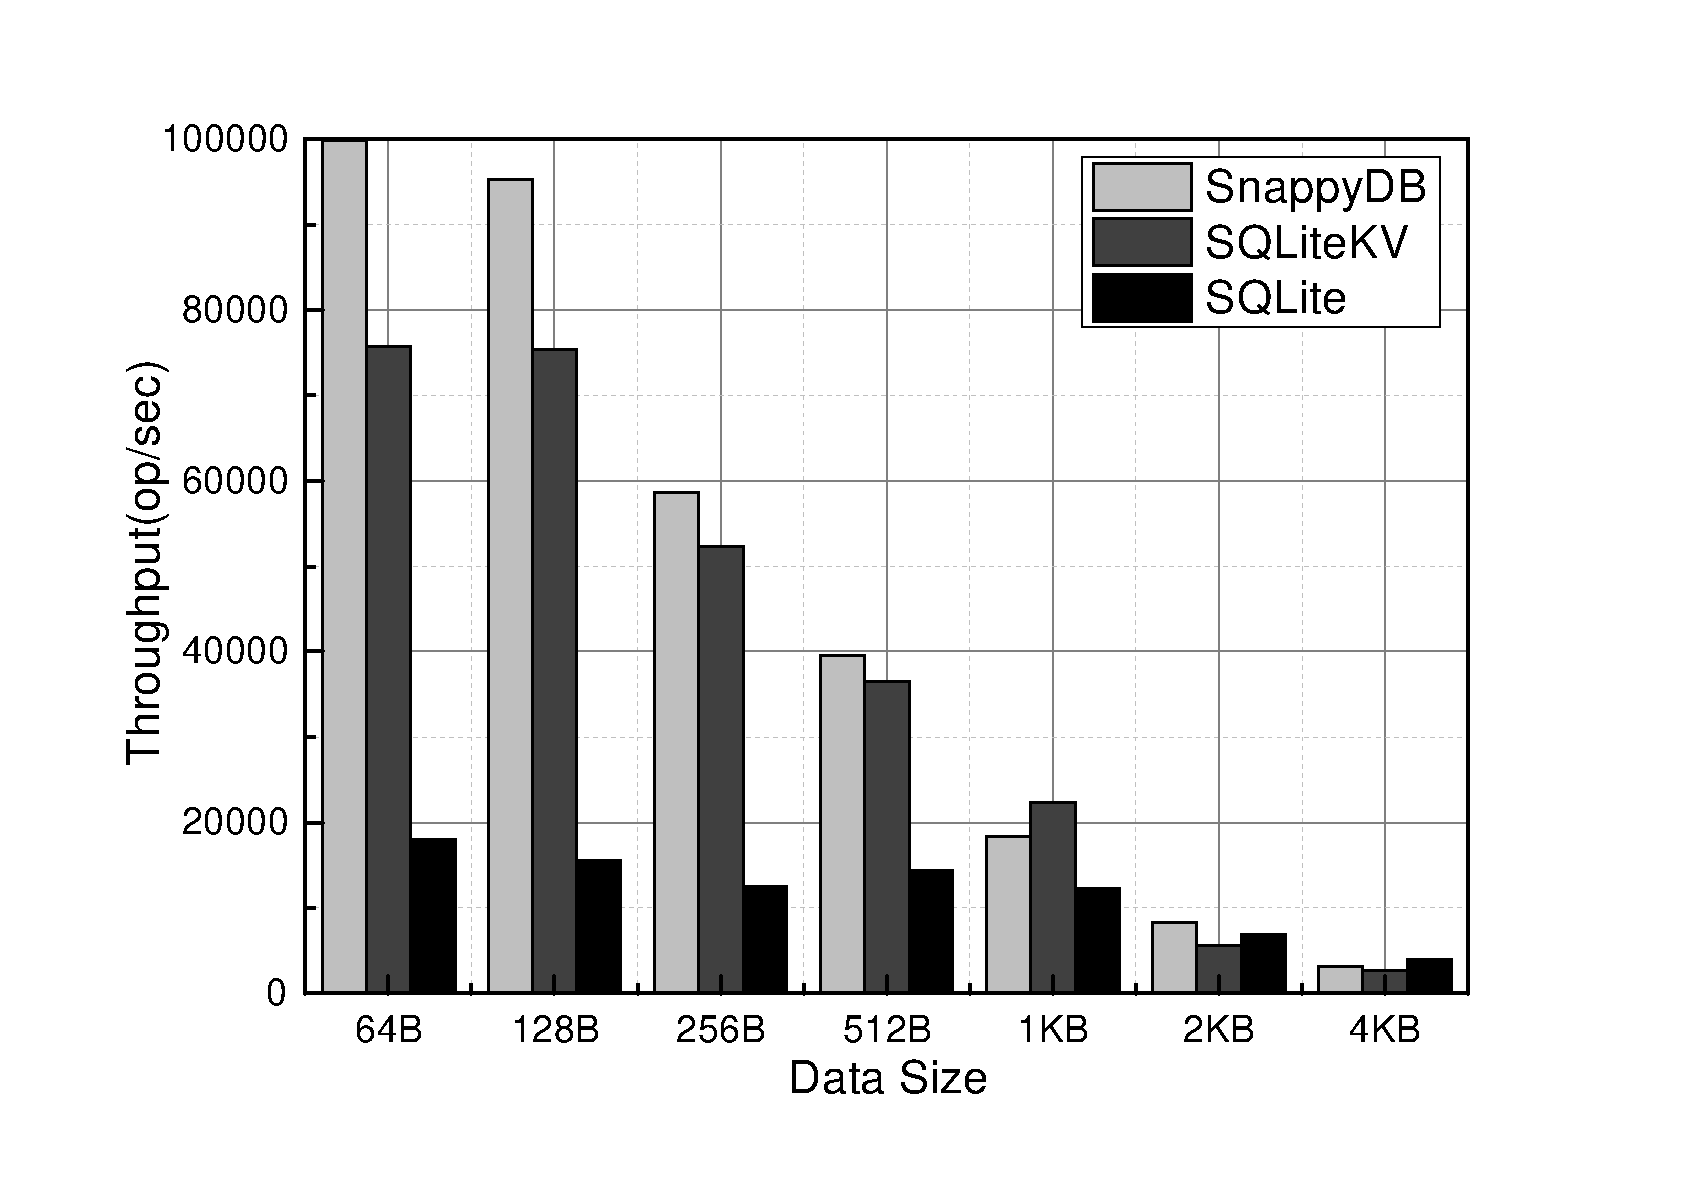
\includegraphics[width=0.9\textwidth, height=3.5cm]{Ext/R-Write.pdf}
		\caption{\small Random Insertions.}
		\label{fig:R-write}
	\end{subfigure}
	\hspace{0.7cm}
	\begin{subfigure}[b]{0.4\textwidth}
		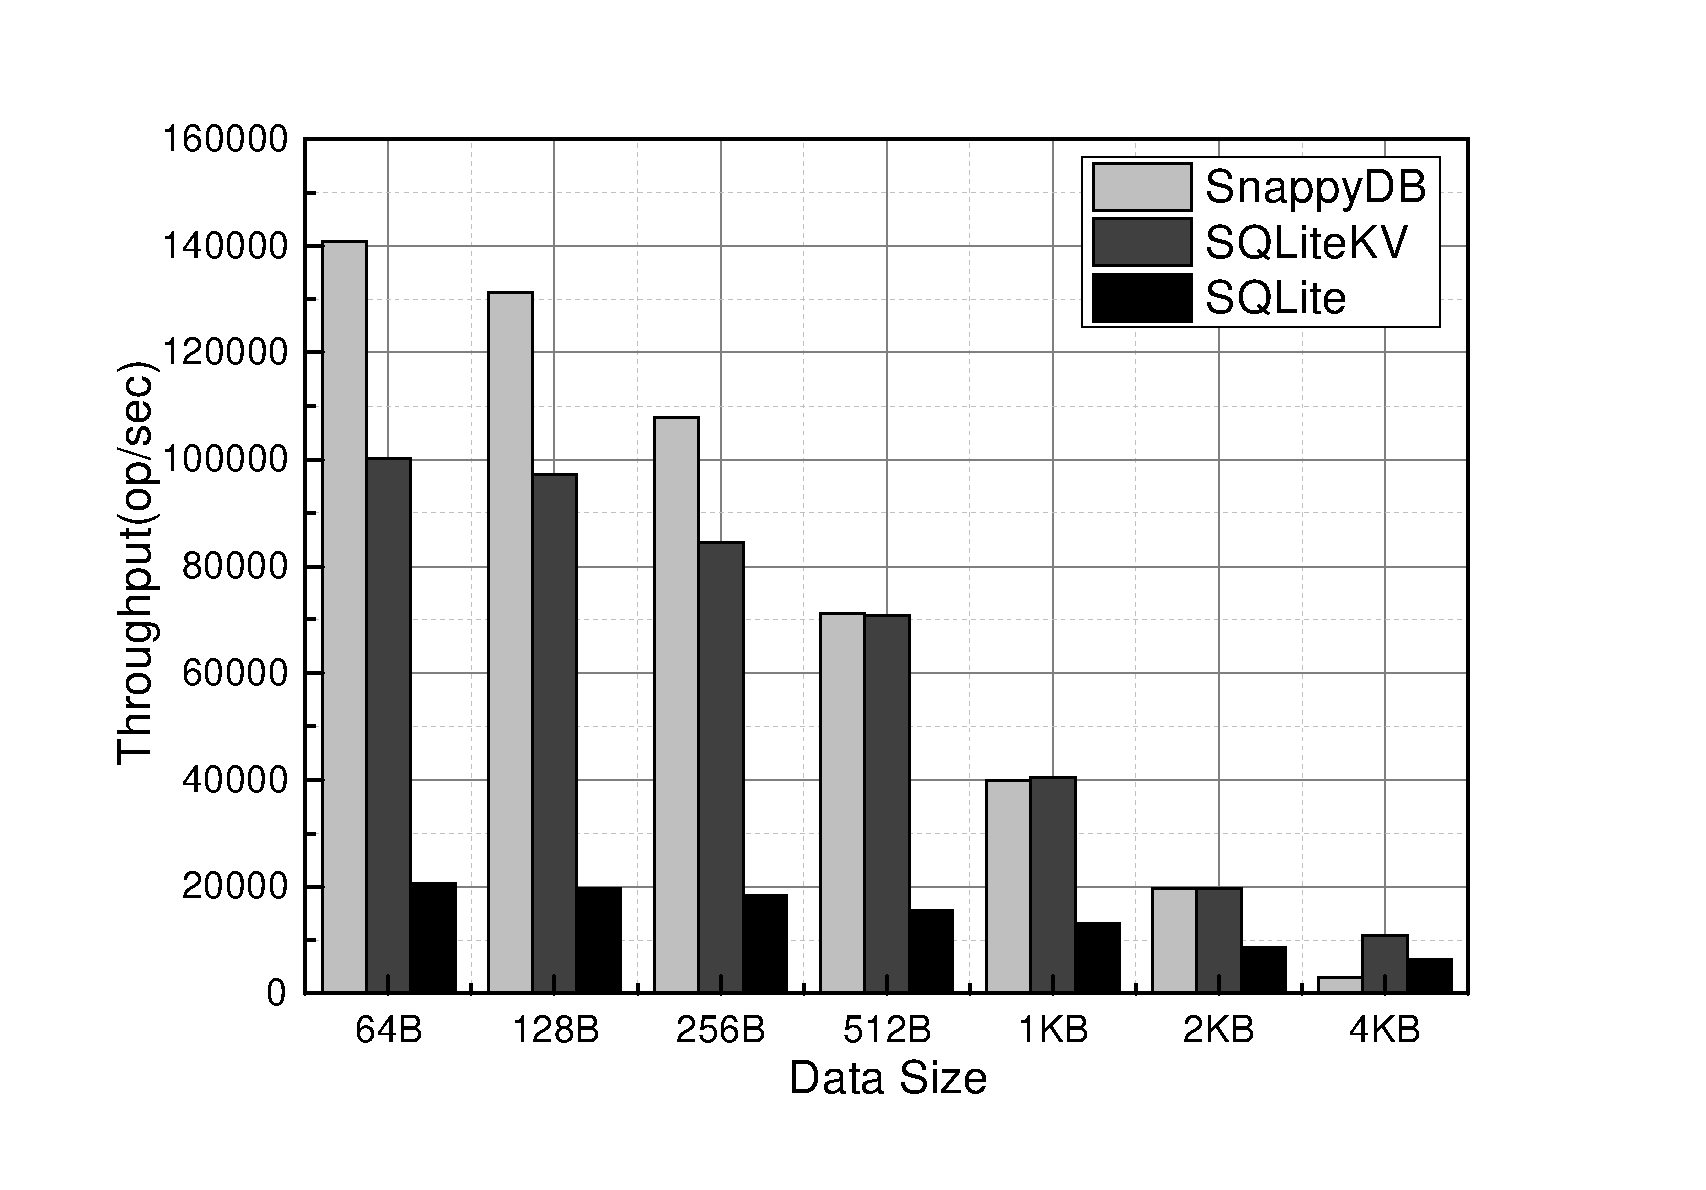
\includegraphics[width=0.9\textwidth, height=3.5cm]{Ext/S-Write.pdf}
		\caption{\small Sequential Insertions.}
		\label{fig:S-write}
	\end{subfigure}
	\caption{\small Insertion Throughput vs. KV size}
\end{figure*}

\begin{figure*}
	\centering
	\begin{subfigure}[b]{0.4\textwidth}
		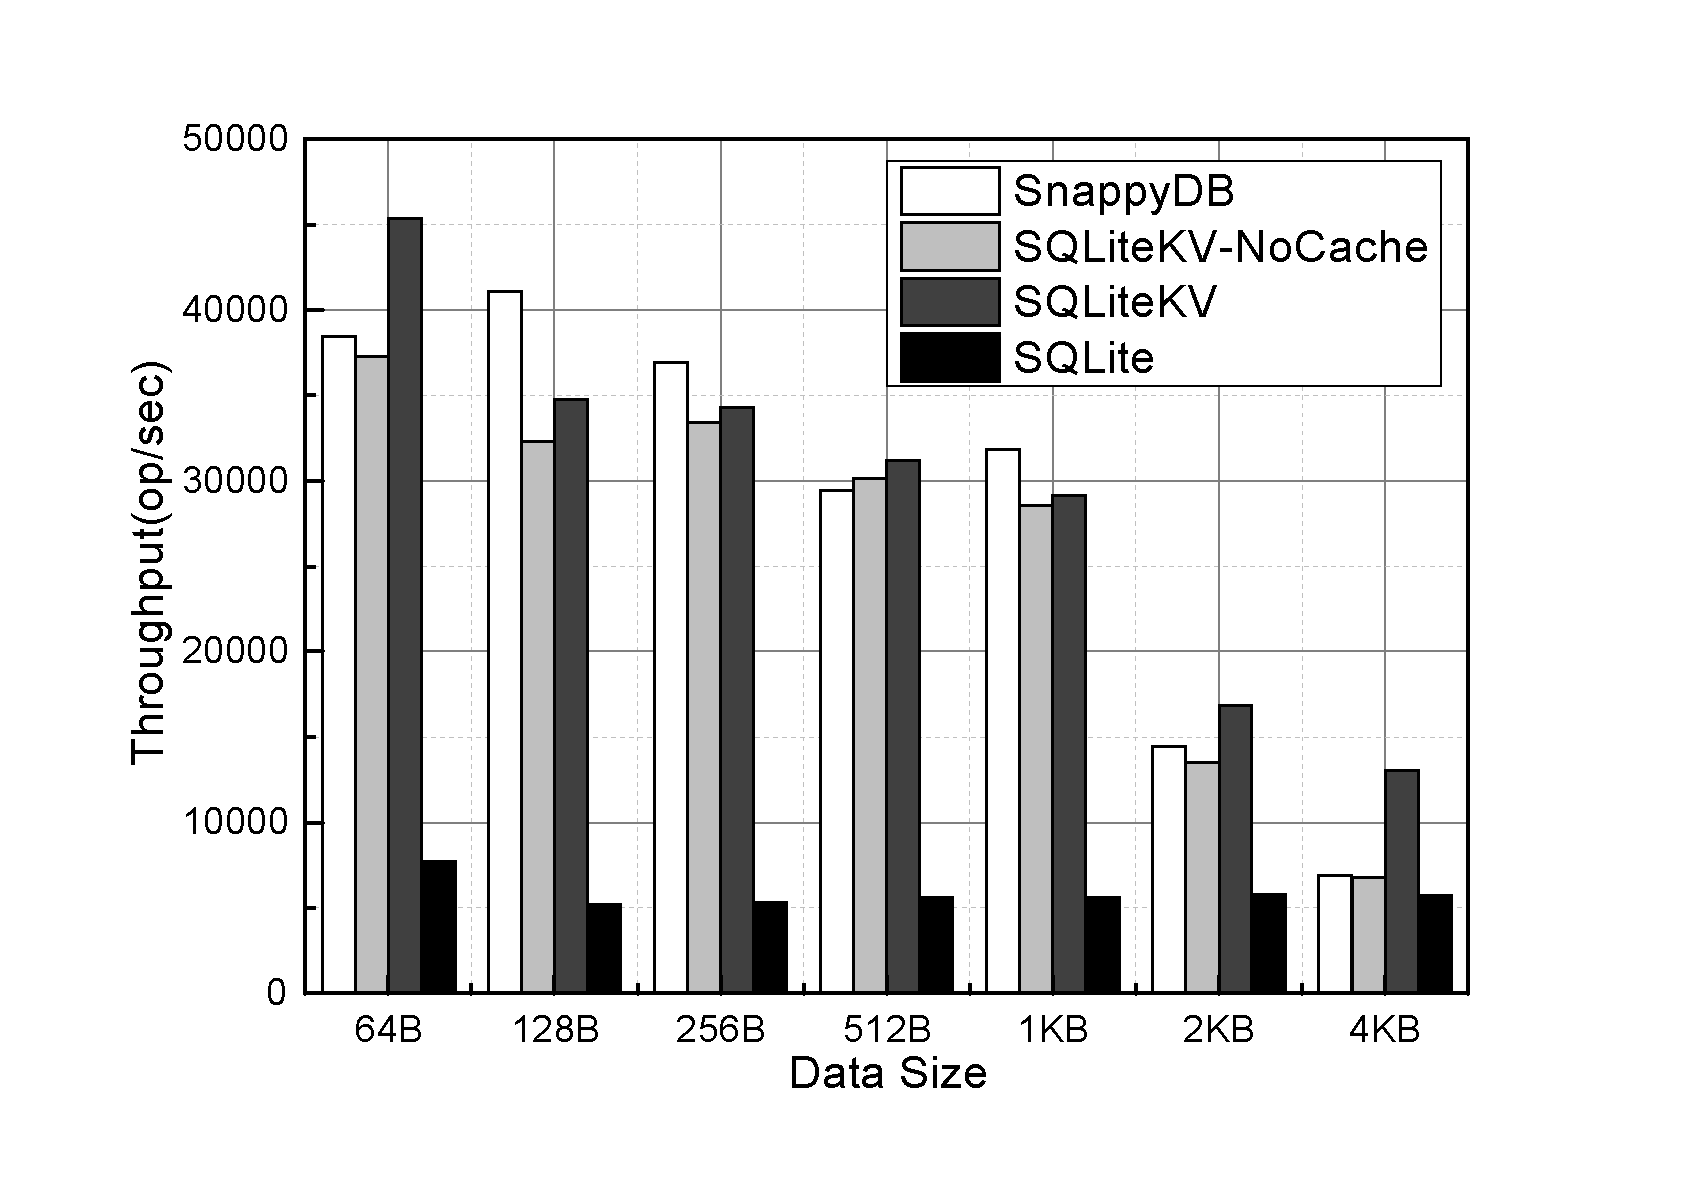
\includegraphics[width=0.9\textwidth, height=3.5cm]{pic/R-read.pdf}
		\caption{\small Random Queries.}
		\label{fig:R-read}
	\end{subfigure}
	\hspace{0.7cm}
	\begin{subfigure}[b]{0.4\textwidth}
		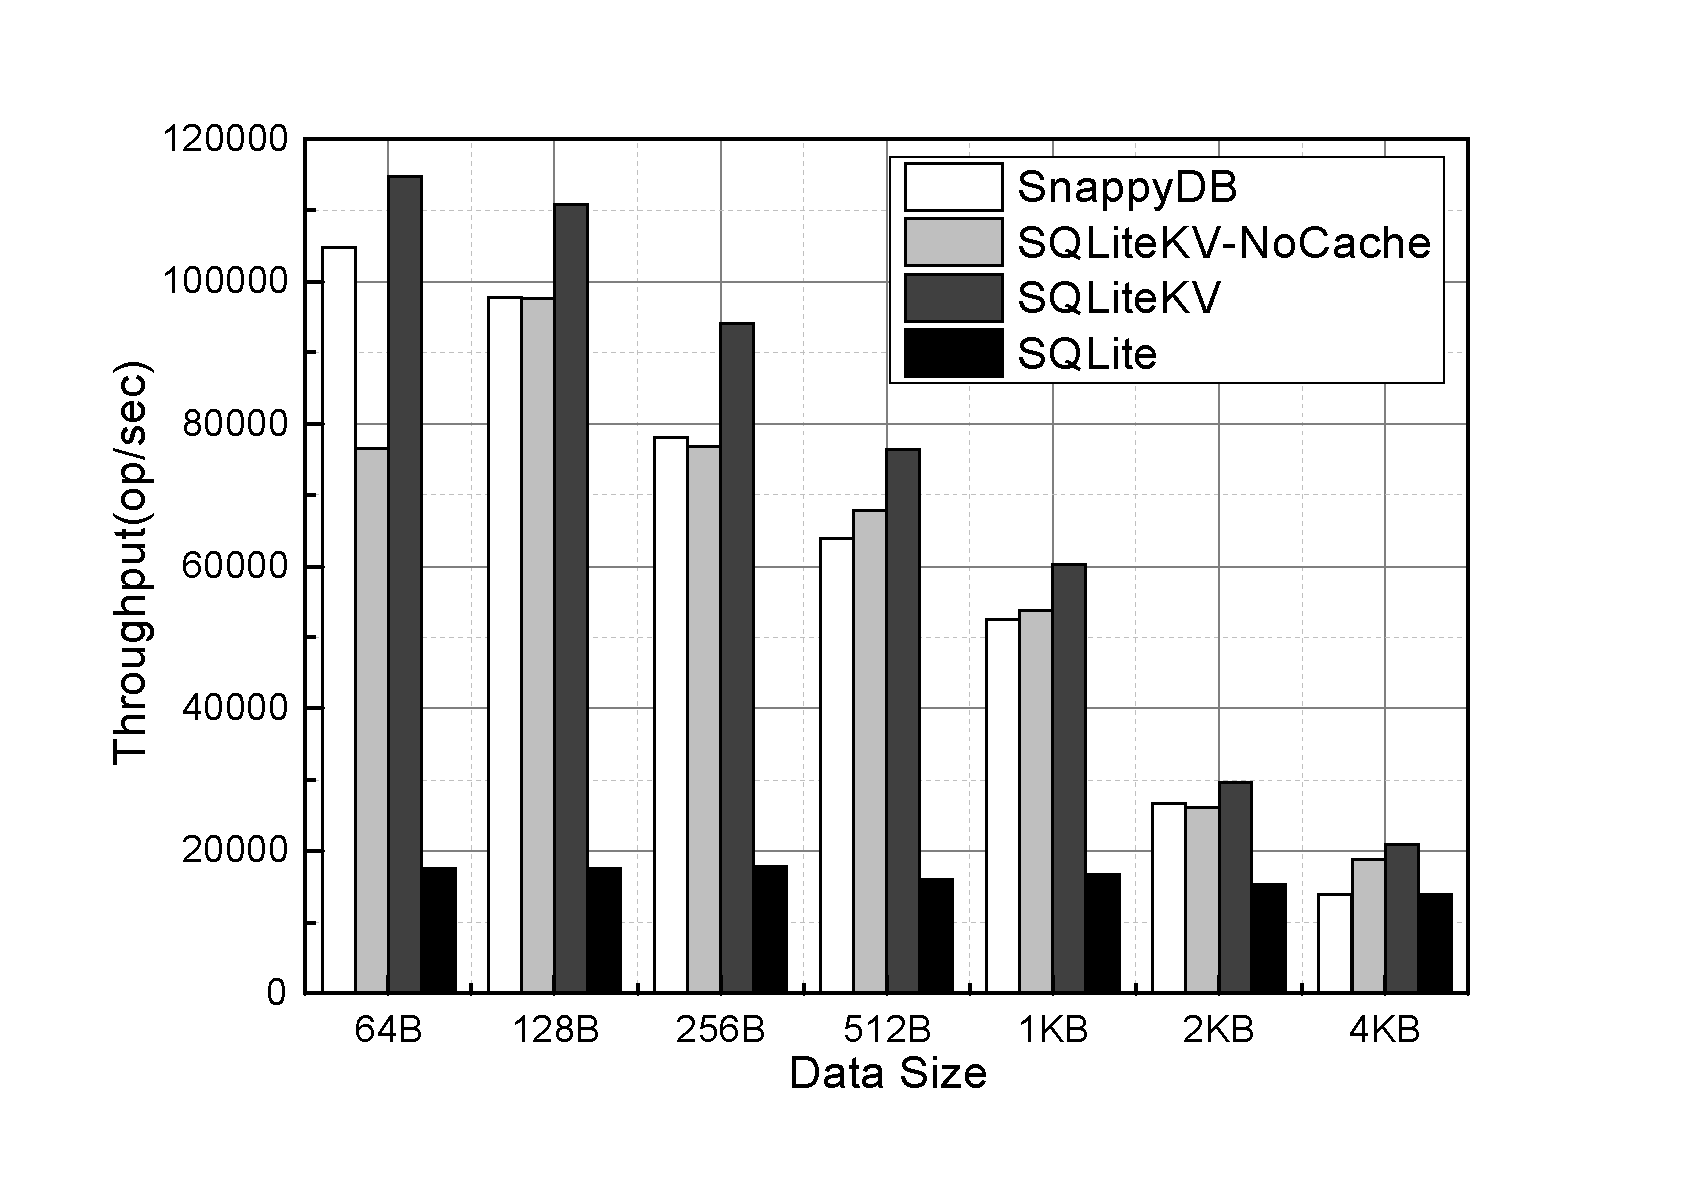
\includegraphics[width=0.9\textwidth, height=3.5cm]{pic/S-read.pdf}
		\caption{\small Sequential Queries.}
		\label{fig:S-read}
	\end{subfigure}
	
	\caption{\small Query Throughput vs. KV size}
	\label{fig:queryPerformance}
\end{figure*}
\subsubsection{Query Performance}
Similarly, Figure ~\ref{fig:S-read} shows the results with random and sequential query operations, respectively. The similar trends can be observed as with insertion operations. Specially, for SQLitKV, its query performance with sequential records is much better than that with random records (the average improvement is around 2 times). 

In Figure ~\ref{fig:S-read}, we also present the results for SQLiteKV without cache. Compared with SQLiteKV, it can observed that our slab-allocation caching mechanism can help improve 10 - 20 \% query performance. Furthermore, it can provide a noteworthy improvement, up to 2.x times, on large data sets.